\documentclass{article}

%%% Fill details here (in the second brackets)
\newcommand{\name}{Weijie Gan}     % Your name (First Last)
\newcommand{\wustlkey}{gan.weijie}             % Your WUSTL Key
%%%



%%%%%%%%%%%%%%%%%%%%%% Formatting Stuff %%%%%%%%%%%%%%%%%%%%%%%%%%%
\usepackage{times}
\usepackage[T1]{fontenc}

\setlength{\parskip}{1em}\setlength{\parindent}{0pt}
\linespread{1.25}
\usepackage[margin=0.7in,top=1in]{geometry}\usepackage{fancyhdr}
\pagestyle{fancy}\lhead{\bf \name}\rhead{\bf \wustlkey}\cfoot{\thepage}
\newcommand{\info}{\clearpage \subsection*{Information}}
\newcommand{\solution}[1]{\clearpage \subsection*{Solution #1}}
\newcommand{\spart}[1]{\paragraph{(#1)}}
%%%%%%%%%%%%%%%%%%%%%%%%%%%%%%%%%%%%%%%%%%%%%%%%%%%%%%%%%%%%%%%%%%%


%%% Add any more packages if you want to
\usepackage{amsmath,graphicx}


\begin{document}
%%%%% Main Body goes here

% Begin solution to every problem like this.
\solution{1} 

\spart{a} First, we can reexpress our problem as:
$$
\begin{aligned}
  \hat{x} & = arg \min_x (x-y)^2 + \lambda|x| \\
  \hat{x} & = arg \min_x x^2 -2xy + y^2 + \lambda|x| \\
\end{aligned}
$$
since $y^2$ is not related with this optimization problem,
$$
  \hat{x} = arg \min_x x^2 -2xy + \lambda|x|
$$

To solve this problem, we need to obtain its first-order derivate and second-order derivate.
Let $f(x) = x^2 -2xy + \lambda|x| $
$$
  \begin{aligned}
    \frac{\partial f}{\partial x} & = 2x - 2y + \lambda sgn(x) \\
    \frac{\partial^2 f}{\partial^2 x} & = 2 \\
  \end{aligned}
$$
because $\frac{\partial^2 f}{\partial^2 x} > 0$ for all $x$, $f(x)$ is a convex function.
Let $\frac{\partial f}{\partial x} = 0$, we can get the global minimum.
$$
    2x - 2y + \lambda sgn(x) = 0
$$
We then can divide the problem into two parts based on whether $x$ is greater than zero.

\textbf{Case 1:} $x > 0$,
$$
  \hat{x} = y - \frac{1}{2}\lambda
$$ 
this is only feasible only under condition that right side of equation is non-negative. So,
$$
  \hat{x} = {(y - \frac{1}{2}\lambda)}^{+} = sgn(y){(|y| - \frac{1}{2}\lambda)}^{+}
$$ 

\textbf{Case 2:} $x < 0$,

It's similar with last case,
$$
  \hat{x} = {(y + \frac{1}{2}\lambda)}^{+} = sgn(y){(|y| - \frac{1}{2}\lambda)}^{+}
$$ 

In conclusion, $\hat{x} = sgn(y){(|y| - \frac{1}{2}\lambda)}^{+}$.

\spart{b} Result with $\lambda = 0.58$ is shown as figure [\ref{fig:1b}]
\begin{figure*}[htbp]
  \centering
  \includegraphics[width = .7\textwidth]{./code/outputs/prob1.png}
  \caption{Problem 1 (b)}
  \label{fig:1b}
\end{figure*}

\solution{2}
\spart{a} Result of \textit{Gray World} is shown as figure [\ref{fig:2a1}], figure [\ref{fig:2a2}] and figure [\ref{fig:2a3}].
\begin{figure*}[htbp]
  \centering
  \includegraphics[width = .4\textwidth]{./code/outputs/prob2a_1.png}
  \caption{Problem 2 (a1)}
  \label{fig:2a1}
\end{figure*}

\begin{figure*}[htbp]
  \centering
  \includegraphics[width = .4\textwidth]{./code/outputs/prob2a_2.png}
  \caption{Problem 2 (a2)}
  \label{fig:2a2}
\end{figure*}

\begin{figure*}[htbp]
  \centering
  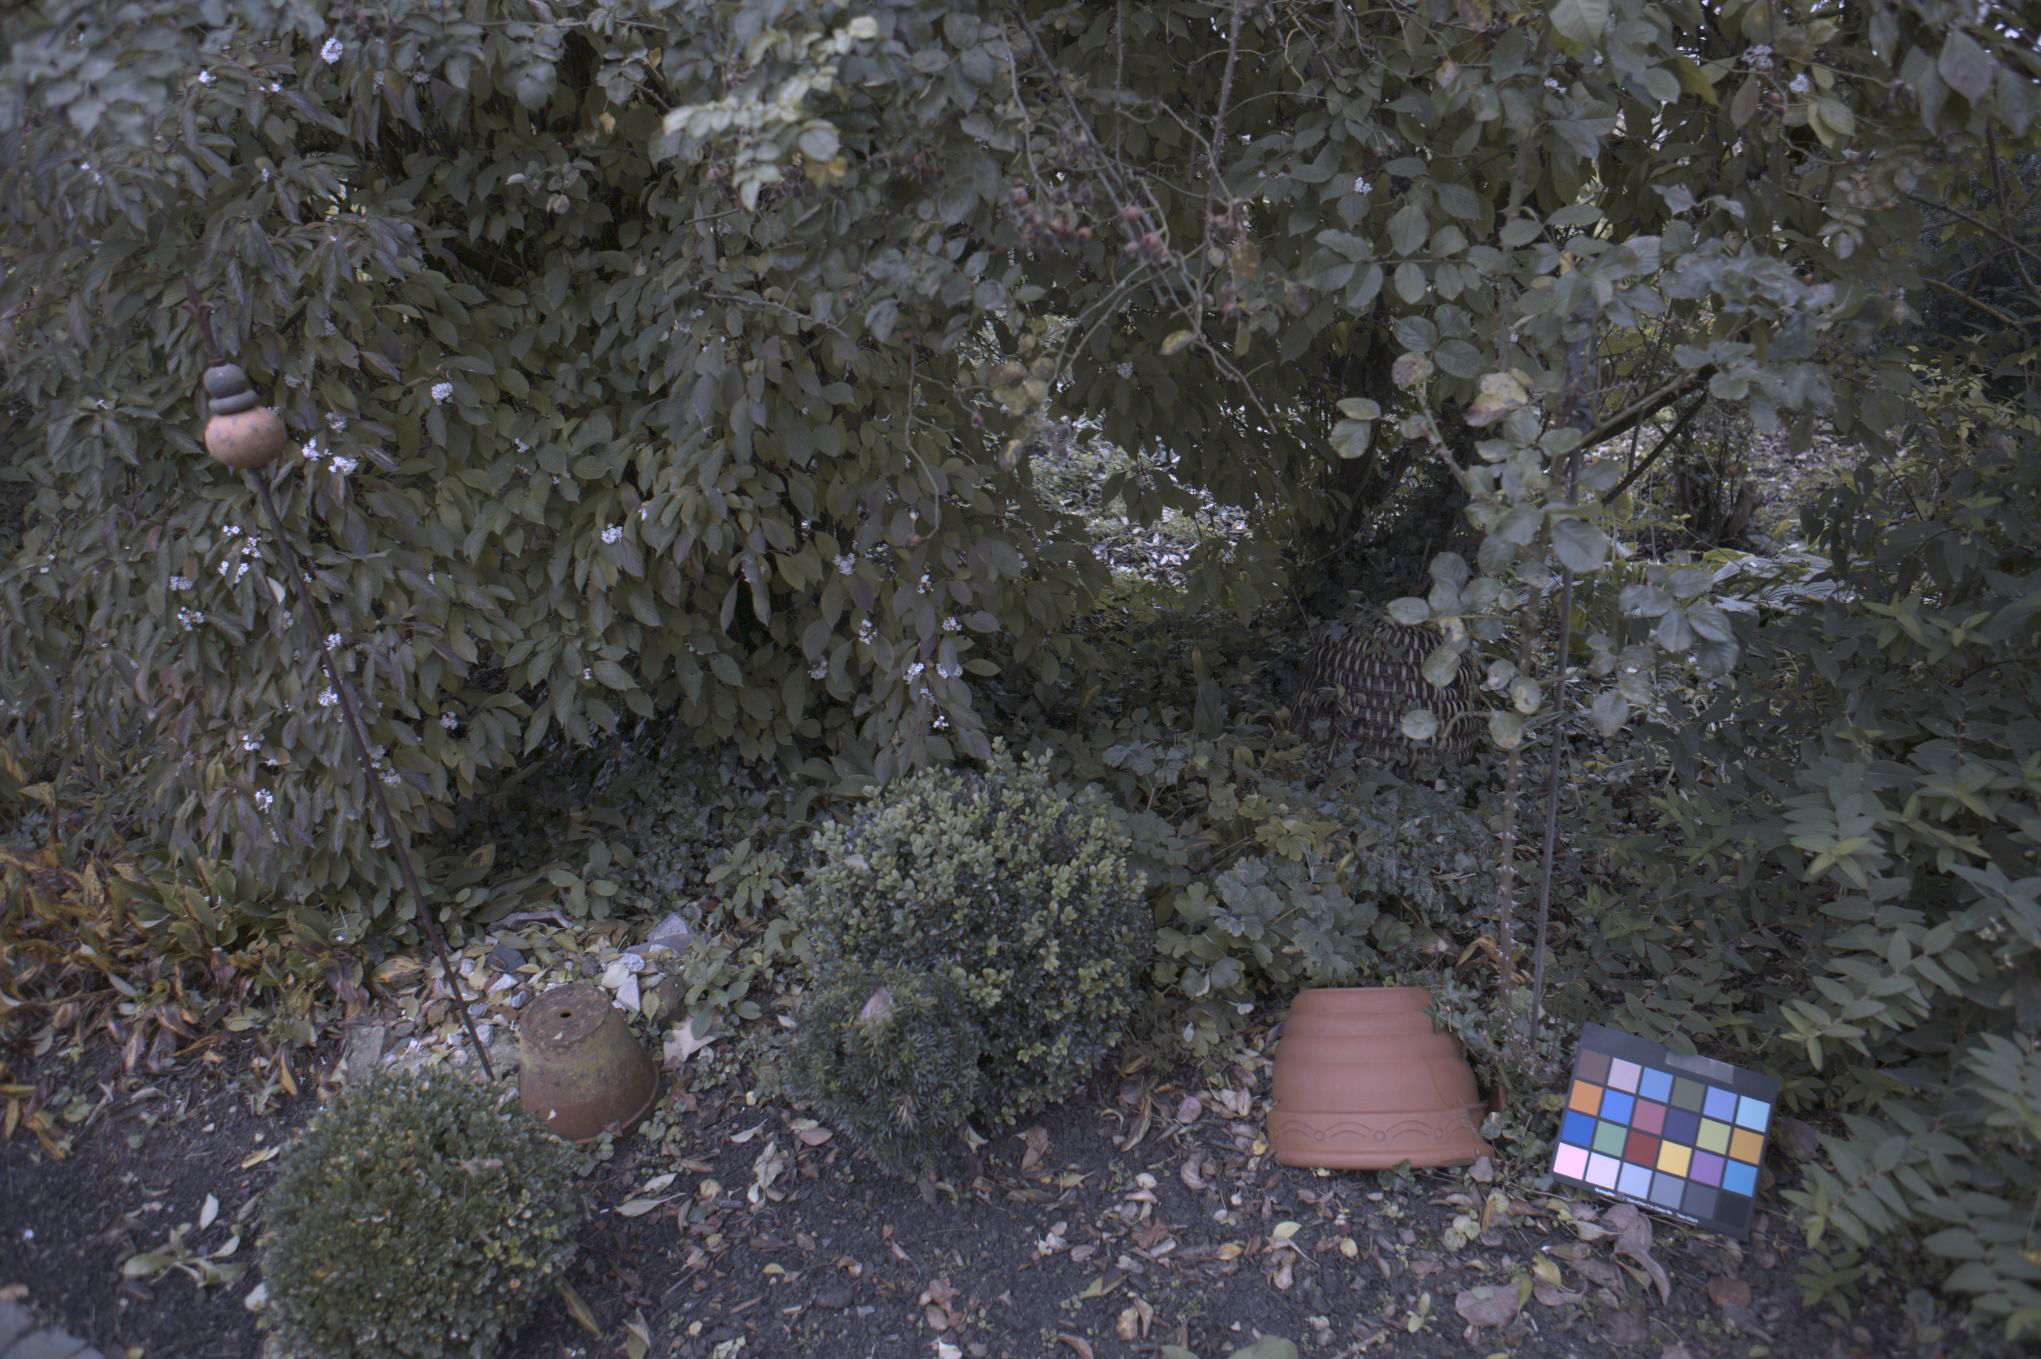
\includegraphics[width = .4\textwidth]{./code/outputs/prob2a_3.png}
  \caption{Problem 2 (a3)}
  \label{fig:2a3}
\end{figure*}

\spart{b} Result of \textit{Gray World with 10\% brightest intensities} is shown as figure [\ref{fig:2b1}], figure [\ref{fig:2b2}] and figure [\ref{fig:2b3}].
\begin{figure*}[htbp]
  \centering
  \includegraphics[width = .4\textwidth]{./code/outputs/prob2b_1.png}
  \caption{Problem 2 (b1)}
  \label{fig:2b1}
\end{figure*}

\begin{figure*}[htbp]
  \centering
  \includegraphics[width = .4\textwidth]{./code/outputs/prob2b_2.png}
  \caption{Problem 2 (b2)}
  \label{fig:2b2}
\end{figure*}

\begin{figure*}[htbp]
  \centering 
  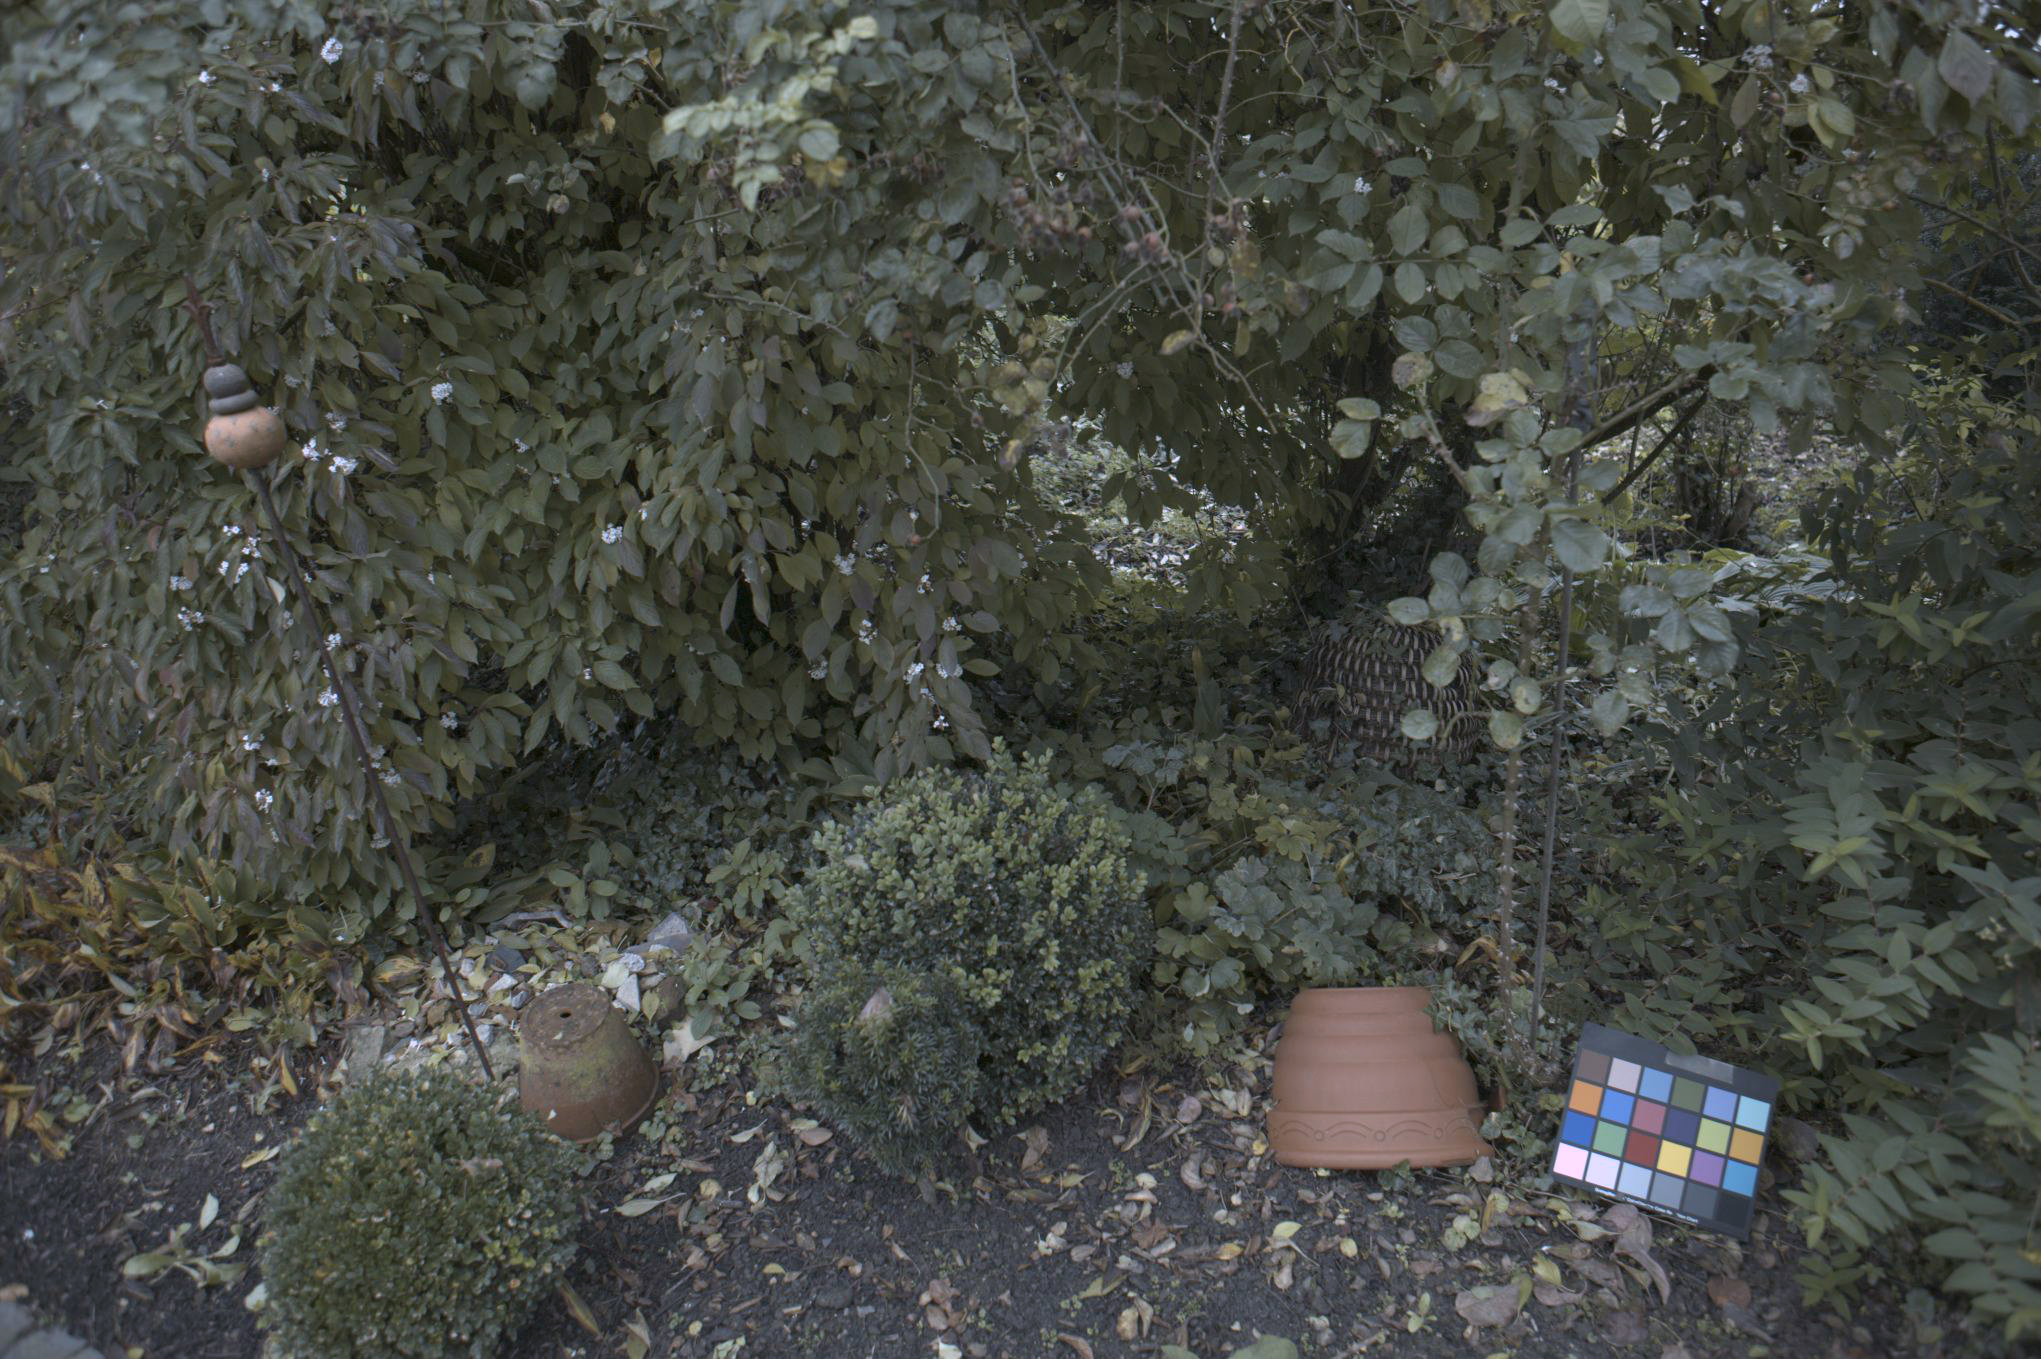
\includegraphics[width = .4\textwidth]{./code/outputs/prob2b_3.png}
  \caption{Problem 2 (b3)}
  \label{fig:2b3}
\end{figure*} 

\solution{3}
\spart{a} Result of normal vector image is shown as figure [\ref{fig:3a}].
\begin{figure*}[htbp]
  \centering 
  \includegraphics[width = .5\textwidth]{./code/outputs/prob3_nrm.png}
  \caption{Problem 3 (a)}
  \label{fig:3a}
\end{figure*} 

\spart{b} Result of surface color albedos image is shown as figure [\ref{fig:3b}].
\begin{figure*}[htbp]
  \centering 
  \includegraphics[width = .4\textwidth]{./code/outputs/prob3_alb.png}
  \caption{Problem 3 (b)}
  \label{fig:3b}
\end{figure*} 

\solution{4}
Result of 3D surface plot image is shown as figure [\ref{fig:4}].
\begin{figure*}[htbp]
  \centering 
  \includegraphics[width = .8\textwidth]{./code/outputs/prob4.png}
  \caption{Problem 4}
  \label{fig:4}
\end{figure*} 

\solution{5}
Result of 3D surface plot image is shown as figure [\ref{fig:5}].
\begin{figure*}[htbp]
  \centering 
  \includegraphics[width = .8\textwidth]{./code/outputs/prob5.png}
  \caption{Problem 5}
  \label{fig:5}
\end{figure*} 

%%%%%%%%%% Important, you must edit and complete the informational
%%%%%%%%%% section below. If you discussed the problem set with no
%%%%%%%%%% one, edit it to say no discussions or external resources.
\info
 
This problem set took approximately 14 hours of effort.

% Note that you might have to escape some special symbols in URLS like \_
I also got hints from the following sources:
\begin{itemize}
\item Derivation of Closed Form Lasso Solution: https://stats.stackexchange.com/questions/17781/derivation-of-closed-form-lasso-solution
\end{itemize}

\end{document}
